\documentclass[12pt]{article}

\usepackage[margin=1in]{geometry}
\usepackage{amsmath,amsthm,amssymb}
\usepackage{mathrsfs}
\usepackage{mathtools}
\usepackage{enumitem}
\usepackage{physics}
\usepackage{pdfpages}
\usepackage{graphicx}
\graphicspath{ {./images/} }

\newcommand{\magsq}[1]{\big|#1\big|^2}
\newcommand{\avg}[1]{\left<#1\right>}
\newcommand{\fullint}[1][x]{\int_{-\infty}^{\infty}\dd #1\;}
\newcommand{\halfint}[1][x]{\int_{0}^{\infty}\dd #1\;}

\begin{document}
	
\title{Final}
\author{Sean Ericson \\ Phys 684}
\maketitle

\section*{Problem 1}
\subsection*{a)}
\subsubsection*{\underline{Problem} (5 points)}
Use momentum conservation to describe briefly how a plane-wave optical field exerts a force on a nearly resonant two-level atom.
What are the direction and amplitude of the force?
What happens if the incident field is not a plane wave?

\subsubsection*{\underline{Solution}}
By Newton's second law, a force is equivalent to a change in momentum over some amount of time. 
By conservation of momentum, when an atom absorbs a photon it receives a change in momentum equal to the momentum of the photon, and similarly when it emits a photon it receives a change in momentum equal and opposite to the photons momentum (this is exactly newton's third law).

The force due to stimulated emission alone averages to zero, as the momentum change from the absorbed photon is cancelled by the momentum change from the emitted photon.
The force due to spontaneous emission alone averages to zero, in this case because spontaneous emission is an isotropic process.

The combined effects of spontaneous and stimulated emission, however, lead to a nonzero force in a direction parallel to the direction of the plane wave wave vector $\vec{k}$, and with amplitude proportional the change in momentum ($\hbar k$) times the average emission rate ($\gamma_2\rho_{22}$).

Even if the incident field is not a plane wave, it can still be decomposed into a sum of plane waves, with the above argument applying to each plane wave component.
Typically, like for a focused laser beam, the component wave vectors will have some amount of divergence, with the overall result being a \textit{gradient} force that acts as a restoring force on the atom.

\subsection*{b)}
\subsubsection*{\underline{Problem} (5 points)}
Discuss briefly how to use a dark state to adiabatically transfer electron population between the two lower states in a a $\Lambda$-type three-level system.
Draw schematically the pulse sequence and the population in the two lower states as a function of time in the adiabatic passage process.
What happens if one does the transfer too fast (i.e. the transfer process is no longer adiabatic)?

\subsubsection*{\underline{Solution}}
The dark state $\ket{D}$ is a superposition of the $\ket{1}$ and $\ket{3}$ states. Specifically,
\[ \ket{D} = \frac{1}{\Omega}\left(\Omega_0'\ket{1} - \Omega_0\ket{3}\right); \quad \Omega = \sqrt{\Omega_0^2 + (\Omega_0')^2}. \]
The dark state is an eigenstate of the Hamiltonian. 
Given that the system starts in this state, we can tune the amplitudes of the fields (sufficiently slowly) such that we remain in the instantaneous eigenstate $\ket{D}$, while changing the particular combination of $\ket{1}$ and $\ket{3}$ that comprise $\ket{D}$.
If initially we have that $\Omega_0 \ll \Omega_0'$, then $\ket{D} \approx \ket{1}$, so the population is effectively in the ground state.
We can then ramp up the field amplitude of $\Omega_0$, while simultaneously ramping down $\Omega_0'$ (again, sufficiently slowly), such that eventually $\ket{D} \approx \ket{3}$.
Thus, we can coherently transfer population from $\ket{1}$ to $\ket{3}$ (or vice-versa, if the sequence is reversed), without exciting the state $\ket{2}$.
\begin{figure}[h!]
    \centering
    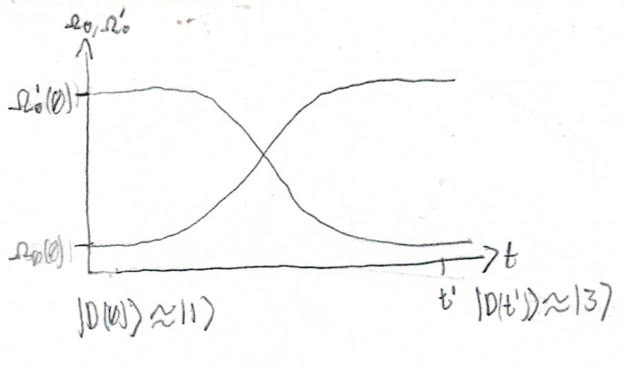
\includegraphics{1b.PNG}
\end{figure}


If the fields are changed too rapidly, such that the adiabatic condition does not hold, the other energy eigenstates of the Hamiltonian (i.e. $\ket{B} = (\Omega_0^*\ket{1} - \Omega_0'^*\ket{3})/\Omega$ and $\ket{2}$) will be excited.

\subsection*{c)}
\subsubsection*{\underline{Problem} (5 points)}
Describe briefly the mechanism of Doppler laser cooling.
What are the limits to Doppler cooling? What is the recoil limit?

\subsubsection*{\underline{Solution}}
As discussed in part (a), the force on a two-level atom subject to a plane wave is proportional to the wave vector, with the maximum average force occurring for a field perfectly resonant with the two-level transition.
For red-detuned counter-propagating waves, atoms moving \textit{against} the direction of either of the waves will see a higher frequency (hence wave vector amplitude) due to the doppler shift, and therefore feel a stronger force than if it were traveling \textit{with} the wave.
Because the waves are counter-propagating, this effect works in both directions and results in an overall dissipative force on the atoms' motion along the axis of the field propagation (i.e. a cooling force).

Spontaneous emission is effectively a heating process that sets a theoretical limit on Doppler cooling.
Even if atoms were cooled to their motional ground state, random kicks from spontaneous emission supply momentum (and thus energy) to the atoms.
The recoil limit represents the temperature associated with the energy due to this process.
Each recoil from spontaneous emission imparts an energy equal to $\hbar^2k^2/2M$ to the atom at a rate given by $\gamma_2\rho_{22}$.
Assuming steady state and using the equipartition theorem, we can associated a temperature with the process of 
\[ T_\text{recoil} \approx \frac{\hbar}{4k_B}\frac{\delta^2 + (\gamma')^2}{\delta} \geq \frac{\hbar\gamma'}{2k_B} \]


\subsection*{d)}
\subsubsection*{\underline{Problem} (5 points)}
Describe briefly pulse propagation under the condition of slow light and electromagnetically induced transparency.
What determines the group velocity in this case?

\subsubsection*{\underline{Solution}}
The inability of the dark state to absorb/emit radiation leads to a suppression of decay/decoherence, which in turn enhances coherent optical interactions.
For the case of EIT (assuming Raman resonance $\delta = \delta'$), near resonance we have that $n \sim \delta \chi'$ where $n$ is the index of refraction.
The dispersion $\chi'$ in the case of EIT exhibits a sharp rise near resonance (i.e. $\dd n/\dd\omega \gg 0$), such that the group velocity
\begin{align*}
    v_g &= \dv{\omega}{k} \\
    &= \frac{1}{\dd k/\dd\omega} \\
    &= \frac{c}{\dv{\omega}(\omega n)} \\
    &= \frac{c}{n + \omega\dv{n}{\omega}} \\
    &\ll c.
\end{align*}
As this effect relies on the coherent interaction between the field and the atoms, lowering $\Omega_0'$ in turns lowering the group velocity, such that $\Omega_0' \to 0 \implies v_g \to 0$.
\begin{figure}[h]
    \centering
    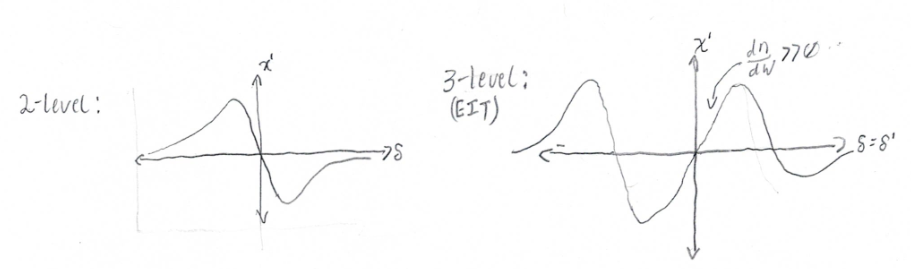
\includegraphics{1d.PNG}
\end{figure}


\subsection*{e)}
\subsubsection*{\underline{Problem} (5 points)}
Discuss briefly the physical mechanism of spectral hole burning and draw schematically a typical hole burning spectral response.
What is the width of the spectral hole?

\subsubsection*{\underline{Solution}}
Spectral hole burning (SHB) is a consequence of the nonlinear component of the susceptibility for a inhomogeneously broadened system in pump-probe spectroscopy. 
Simply put, the pump field saturates the atoms with $\omega_0 \approx \omega_a$, leading to a decrease in the absorption near that frequency measured by the probe field.
We calculated that
\[ \chi_\text{inh}^\text{NL}(\omega_b) \propto \frac{\gamma + \gamma'}{(\omega_a-\omega_b)^2 + (\gamma + \gamma')^2}, \]
from which we can see that the linewidth for SHB is $2(\gamma + \gamma')$, where
\[ \gamma' = \gamma\sqrt{1 + \frac{\abs{\Omega_a}^2}{\gamma\gamma_2}} \]
includes the effects of power broadening.
\begin{figure}[h]
    \centering
    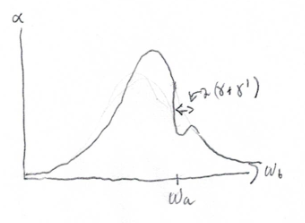
\includegraphics{1e.png}
\end{figure}

\subsection*{f)}
\subsubsection*{\underline{Problem} (5 points)}
Discuss briefly why an inhomogeneously broadened laser medium tends to support multi-mode lasing operation, while a homogeneously broadened laser medium tends to support single-mode lasing operation.

\subsubsection*{\underline{Solution}}
In an inhomogeneously broadened system, there is a range of resonant frequencies among the atoms. Lasing can therefore occur across a range of frequencies (and hence modes).
For a homogeneously broadened system there is only one resonant frequency, and therefore only single-mode lasing is supported.

\section*{Problem 2}
\subsubsection*{\underline{Problem} (25 points)}
In this experiment, we apply three, instead of two, laser pulses to an inhomogeneously broadened two-level system.
All three laser pulses are $\pi/2$ pulses.
We assume that the atoms are initially in the lower state and that the pulses are short and intense such that the effects of detuning and decay can be ignored during each pulse.
The dipole decoherence rate is $\gamma$, and the excited state population decay rate is $\gamma_2$.
\begin{figure}[h]
    \centering
    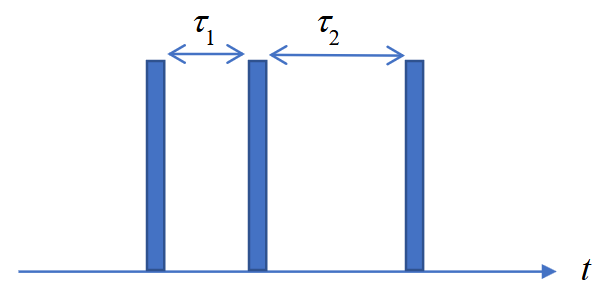
\includegraphics[scale=.75]{spin_echo.png}
\end{figure}
\begin{enumerate}[label=(\alph*)]
    \item Write down the Bloch vector in the $x$-$y$ plane right before the second pulse for an atom with detuning $\delta$ from the applied field.
    \item Write down the $z$ component of the Bloch vector for the above atom right after the second pulse.
    \item Write down the $z$ component of the Bloch vector right before the third pulse.
    \item Write down the Bloch vector in the $x$-$y$ plane right after the third pulse, \textit{including only the contribution due to the $z$ component in (c)}.
    \item An echo forms after the third pulse. What is the timing of the echo and why?
    \item Compared with the usual two-pulse echo, what additional information can we obtain with the three-pulse echo (assuming that you can measure the echo intensity as a function of $\tau_1$ and $\tau_2$)?
\end{enumerate}

\subsubsection*{\underline{Solution}}
\begin{enumerate}[label=(\alph*)]
    \item The first pulse (which affects a rotation of $\pi/2$ about the $\hat{x}$ axis) takes the Bloch vector from its initial state ($\hat{z}$) to the $\hat{y}$ axis.
    Neglecting decay, free evolution (i.e. rotation about the $\hat{z}$ axis at rate $\delta$) occurs in the period between the first and second pulse, so just before the second pulse the Bloch vector is in the state $\vec{R} = -\sin(\delta\tau_1)\hat{x} + \cos(\delta\tau_1)\hat{y}$.
    To include decay, we note that
    \[
    \begin{rcases*}
        \dot{u} = -\gamma u \\
        \dot{v} = -\gamma v \\
        \dot{w} = -\gamma_2(w + 1)
    \end{rcases*}
    \implies
    \begin{aligned}
        u(t) &= u_0e^{-\gamma t} \\
        v(t) &= v_0e^{-\gamma t} \\
        w(t) &= (w_0 + 1)e^{-\gamma_2 t} - 1.
    \end{aligned} 
    \]
    So, including this decay, we have that
    \[ \vec{R} = \mqty(-\sin(\delta\tau_1)e^{-\gamma\tau_1} \\ \cos(\delta\tau_1)e^{-\gamma \tau_1} \\ e^{-\gamma_2\tau_1} - 1) \]
    immediately before the second pulse.
    \item The second pulse is again a rotation about $\hat{x}$ by $\pi/2$, which has the effect of taking $\hat{y}\to\hat{z}, \; \hat{z}\to-\hat{y}$. 
    Thus, the $z$ component of the Bloch vector immediately after the second pulse is simply the $y$ component before the pulse, i.e. $\cos(\delta\tau_1)e^{-\gamma\tau_1}$.
    \item Between the second and third pulses, free evolution (rotation about $\hat{z}$) occurs, so the only change to the $z$ component is due to decay, i.e. the $z$ component is now
    \begin{align*}
        R_z &= (\cos(\delta\tau_1)e^{-\gamma\tau_1} + 1)e^{-\gamma_2\tau_2} - 1 \\
        &= \cos(\delta\tau_1)e^{-\gamma\tau_1 - \gamma_2\tau_2} + e^{\gamma_2\tau_2} - 1
    \end{align*}
    \item As stated previously the $\pi/2$ pulses take $\hat{z}\to-\hat{y}$, so, considering only the $z$ component from the previous part, the Bloch vector is in the state $\left(\cos(\delta\tau_1)e^{-\gamma\tau_1 - \gamma_2\tau_2} + e^{\gamma_2\tau_2} - 1\right)\hat{y}$.
    \item  
    \item 
\end{enumerate}


\section*{Problem 3}
\subsubsection*{\underline{Problem} (25 points)}
We consider a cascaded 3-level system, where one laser beam $E$ with frequency $\omega$ interacts with the $\ket{1}\leftrightarrow\ket{2}$ dipole transition and another laser beam $E'$ with frequency $\omega'$ interacts with the $\ket{2}\leftrightarrow\ket{3}$ dipole transition, as shown schematically in the figure.
Assume that initially the atom is in the ground state (state $\ket{1}$), decay rates for population in $\ket{2}$ and $\ket{3}$ are $\gamma_2$ and $\gamma_3$, respectively, and decay rates for $\rho_{12}$, $\rho_{23}$ and $\rho_{13}$ are $\gamma_{12}$, $\gamma_{23}$ and $\gamma_{13}$, respectively.
For simplicity, we also assume that the Rabi frequencies for the two dipole transitions, $\Omega_0$ and $\Omega_0'$, are real.
\begin{figure}[h]
    \centering
    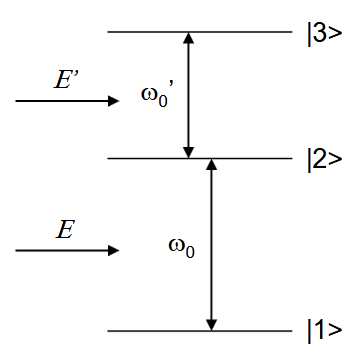
\includegraphics[scale=.75]{cascade.png}
\end{figure}
\begin{enumerate}[label=(\alph*)]
    \item Write down the wave function in the field-interaction representation, for which the Hamiltonian will have no explicit time dependence. Use this wave function to derive or write down the Hamiltonian in the field-interaction representation.
    \item Derive the density matrix equation for the nonradiative coherence, i.e., $\rho_{13}$.
    \item Assuming that laser beam $E'$ can be strong, but laser beam $E$ is weak, write down the relevant density matrix equations that you will need in order to calculate the susceptibility probed by the weak laser beam $E$.
    \item Calculate the susceptibility probed by laser beam $E$.
    \item Under what conditions will the system remain approximately in the ground state even when $E$ is nearly resonant with the atomic transition? Explain briefly the underlying physics.
    \item Discuss briefly the main difference between the $\Lambda$-type and the cascaded-type 3-level systems.
\end{enumerate}

\subsubsection*{\underline{Solution}}
\begin{enumerate}[label=(\alph*)]
    \item The field-interaction representation factors-out the evolution of the applied fields via
    \[ \ket{\psi(t)} = \tilde{c}_1(t)e^{i\omega t}\ket{1} + \tilde{c}_2\ket{2} + \tilde{c}_3e^{-\omega't}\ket{3}, \]
    i.e. using the transformation
    \[ c_1 \to \tilde{c}_1 = c_1e^{-i\omega t}; \quad c_2 \to \tilde{c}_2 = c_2; \quad c_3 \to \tilde{c_3} = c_3e^{-i\omega't}. \]
    Then,
    \begin{align*}
        \dot{\tilde{c}}_1 &= \left(-i\omega c_1 + \dot{c}_1\right)e^{-i\omega t} \\
        &= \left(-i\omega c_1 + i\omega_0c_1 - \frac{i}{2}\Omega_0e^{i\omega t}\right)e^{-i\omega t} \\
        &= i\delta\tilde{c}_1 - \frac{i}{2}\Omega_0\tilde{c}_2 \\
        \dot{\tilde{c}}_2 &= -\frac{i}{2}\left(\Omega_0\tilde{c}_1 + \Omega_0'\tilde{c}_3\right) \\
        \dot{\tilde{c}}_3 &= \left(i\omega'c_3 + \dot{c}_3\right)e^{i\omega't} \\
        &= \left(-i\omega'c_3 + -\frac{i}{2}\Omega_0'e^{-i\omega't}c_2 + i\omega_0'c_3\right)e^{i\omega't} \\
        &= -\frac{i}{2}\Omega_0' \tilde{c}_2 + i\delta'\tilde{c}_3.
    \end{align*}
    Putting this together, we have
    \begin{alignat*}{3}
        &\quad & \partial_t \tilde{\ket{\psi}} &= i\mqty(\delta\tilde{c}_1 - \frac{1}{2}\Omega_0\tilde{c}_2 \\ -\frac{1}{2}\Omega_0\tilde{c}_1 - \frac{1}{2}\Omega_0'\tilde{c}_3 \\ -\frac{1}{2}\Omega_0'\tilde{c}_2 + \delta'\tilde{c}_3) \\
        &\quad & &= -\frac{i}{\hbar}\tilde{H}\tilde{\ket{\psi}} \\
        &\implies\quad & \tilde{H} &= \hbar\mqty(-\delta & \frac{\Omega_0}{2} & 0 \\ \frac{\Omega_0}{2} & 0 & \frac{\Omega_0'}{2} \\ 0 & \frac{\Omega_0'}{2} & -\delta').
    \end{alignat*}
    \item Since $\rho = \dyad{\psi}$, we have that $\tilde{\rho}_{13} = \tilde{c}_1\tilde{c}_3^*$, so
    \begin{alignat*}{3}
        &\quad & \tilde{\rho}_{13} &= \tilde{c}_1\tilde{c}_3^* \\
        &\implies & \dot{\tilde{\rho}}_{13} &= \dot{\tilde{c}}_1\tilde{c}_3^* + \tilde{c}_1\dot{\tilde{c}}_3^* \\
        & & &= \left(i\delta\tilde{c}_1 - \frac{i}{2}\Omega_0\tilde{c}_2 \right)\tilde{c}_3^* + \tilde{c}_1\left(\frac{i}{2}\Omega_0' \tilde{c}_2 - i\delta'\tilde{c}_3\right) \\
        & & &= i\delta\tilde{\rho}_{13} - \frac{i}{2}\Omega_0\tilde{\rho}_{23}  + \frac{i}{2}\Omega_0' \tilde{\rho}_{12} - i\delta'\tilde{\rho}_{13} \\
        & & &= i(\delta - \delta')\tilde{\rho}_{13} - \frac{i}{2}\Omega_0\tilde{\rho}_{23}  + \frac{i}{2}\Omega_0' \tilde{\rho}_{12}
    \end{alignat*}
    We need to include decay, but this just means inserting the term $-\gamma_{13}\tilde{\rho}_{13}$ into the equation of motion for $\tilde{\rho}_{13}$, so, finally,
    \[ \dot{\tilde{\rho}}_{13} = \left[i(\delta - \delta') - \gamma_{13}\right]\tilde{\rho}_{13} - \frac{i}{2}\Omega_0\tilde{\rho}_{23}  + \frac{i}{2}\Omega_0' \tilde{\rho}_{12} \]
    \item To calculate the susceptibility probed by the weak $E$ field (which couples to the $\ket{1}\Leftrightarrow\ket{2}$ transitions), we will need to know $\tilde{\rho}_{12}$.
    Following the same procedure as above,
    \begin{alignat*}{3}
        &\quad & \tilde{\rho}_{12} &= \tilde{c}_1\tilde{c}_2^* \\
        &\implies & \dot{\tilde{\rho}}_{12} &= \dot{\tilde{c}}_1\tilde{c}_2^* + \tilde{c}_1\dot{\tilde{c}}_2^* \\
        & & &= \left(i\delta\tilde{c}_1 - \frac{i}{2}\Omega_0\tilde{c}_2\right)\tilde{c}_2 + \tilde{c}_1\left(\frac{i}{2}\left(\Omega_0\tilde{c}_1 + \Omega_0'\tilde{c}_3\right)\right) \\
        & & &= i\delta\tilde{\rho}_{12} - \frac{i}{2}\Omega_0\tilde{\rho}_{22} + \frac{i}{2}\left(\Omega_0\tilde{\rho}_{11} + \Omega_0'\tilde{\rho}_{13}\right) \\ 
        & & &= i\delta\tilde{\rho}_{12} - \frac{i}{2}\Omega_0\left(\tilde{\rho}_{22}-\tilde{\rho}_{11}\right) + \frac{i}{2}\Omega_0'\tilde{\rho}_{13} \\
        & & &\to \left(i\delta - \gamma_{12}\right)\tilde{\rho}_{12} - \frac{i}{2}\Omega_0\left(\tilde{\rho}_{22}-\tilde{\rho}_{11}\right) + \frac{i}{2}\Omega_0'\tilde{\rho}_{13},
    \end{alignat*}
    where in the last line we've included decay. This equation contains $\tilde{\rho}_{11}$ and $\tilde{\rho}_{22}$, so we'll also need their equations of motion:
    \begin{align*}
        \dot{\tilde{\rho}}_{11} &= \dot{\tilde{c}}_1\tilde{c}_1^* + \tilde{c}_1\dot{\tilde{c}}_1^* \\
        &= 2\Re[\dot{\tilde{c}}_1\tilde{c}_1^*] \\
        &= 2\Re\left[\left(i\delta\tilde{c}_1 - \frac{i}{2}\Omega_0\tilde{c}_2\right)\tilde{c}_1^*\right] \\
        &= \Omega_0 \Im\left[\tilde{\rho}_{21}\right] \\
        &= -\frac{i}{2}\Omega_0\left(\tilde{\rho}_{21} - \tilde{\rho}_{12}\right) \\
        &\to -\frac{i}{2}\Omega_0\left(\tilde{\rho}_{21} - \tilde{\rho}_{12}\right) - \gamma_1\tilde{\rho}_{11},
        \\ \\
        \dot{\tilde{\rho}}_{22} &= 2\Re[\dot{\tilde{c}}_2\tilde{c}_2^*] \\
        &= 2\Re\left[-\frac{i}{2}\left(\Omega_0\tilde{c}_1 + \Omega_0'\tilde{c}_3\right)\tilde{c}_2^*\right] \\
        &= \Omega_0\Im\left[\tilde{\rho}_{12}\right] + \Omega_0'\Re\left[\tilde{\rho}_{32}\right] \\
        &= -\frac{i}{2}\Omega_0\left(\tilde{\rho}_{12} - \tilde{\rho}_{21}\right) + \frac{1}{2}\Omega_0'\left(\tilde{\rho}_{32} + \tilde{\rho}_{23}\right) \\
        &\to -\frac{i}{2}\Omega_0\left(\tilde{\rho}_{12} - \tilde{\rho}_{21}\right) + \frac{1}{2}\Omega_0'\left(\tilde{\rho}_{32} + \tilde{\rho}_{23}\right) - \gamma_2\tilde{\rho}_{22}
    \end{align*}
    \item Since the probe field is weak, we can calculate the susceptibility to first order in $\Omega_0$
    \item If the decay rate $\gamma_2$ is large, this will contribute to keeping the system approximately in the ground state, as excitations of the $\ket{2}$ state will quickly decay back to the $\ket{1}$ state.
    If the Rabi frequency $\Omega_0'$ is not particularly large (compared to $\gamma_2$), then population will not have time to transition from $\ket{2}$ to $\ket{3}$ before decaying from $\ket{2}$ to $\ket{1}$, therefore helping to maintain the excitation in state $\ket{1}$.
    Additionally, if $\Omega_0' \gg \Omega_0$, the dark state $\ket{D} = \frac{1}{\Omega}\left(\Omega_0'\ket{1} - \Omega_0\ket{3}\right) \approx \ket{1}$. Coherent population trapping then maintains this state, keeping the system approximately in the ground state.
    \item Since the $\ket{3}$ state has a lower energy in than the $\ket{2}$ state in the $\Lambda$-type system (and transitions between the $\ket{1}$ and $\ket{3}$ states are dipole-forbidden), the $\ket{3}$ state is considerably more stable in the $\Lambda$-type system than in the cascade-type system.
    This results in significantly lower decay rates, and correspondingly stronger and longer-lasting coherence (particularly the dipole coherences $\tilde{\rho}_{23}$ and $\tilde{\rho}_{23}$), which in turn allows for the neat features we studied such as stimulated Raman adiabatic passage and slow light.
\end{enumerate}


\section*{Problem 4}
\subsubsection*{\underline{Problem} (20 points)}
Consider the transitions form the ground state with total angular momentum $J=0$ to the excited states with $J=1$ (see the figure below). The atom (which is near $z=0$) is put in a magnetic field gradient along the $z$-direction with $B=\beta z$ where $\beta$ is a positive constant. 
Assume that the magnetic sublevels' energies vary as $E_m = E_0 + gmz$, where $g$ is a positive constant and $m$ is the magnetic quantum number.

For this experiment, we apply two counter propagating laser beams (for simplicity, assume the laser beams are plane waves) with the same frequency and opposite circular polarization to the atom.
The $\sigma_+$ laser beam (coupling to the $J=0$ to $m=1$ transition) is incident in the $+z$ direction and the $\sigma_-$ laser beam (coupling to the $J=0$ to $m=-1$ transition) is incident in the $-z$ direction.
The two transitions have the same spontaneous emission rate, $\gamma_2$, and the same Rabi frequency, $\Omega_0$
\begin{figure}[h]
    \centering
    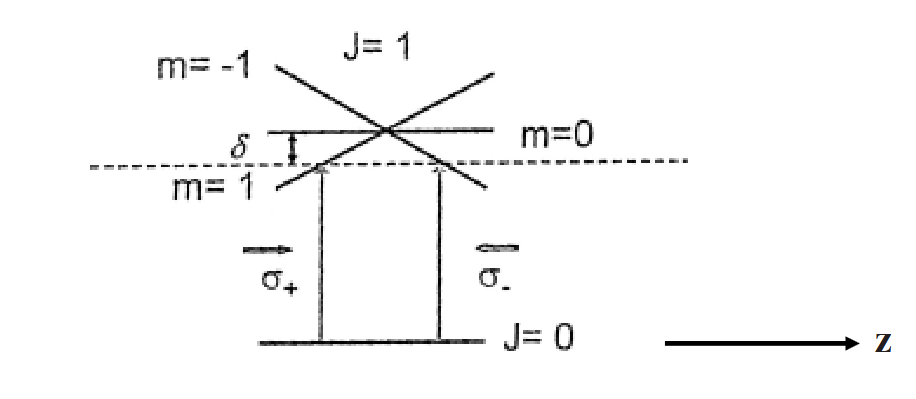
\includegraphics[scale=.75]{polarized_beams.png}
\end{figure}
\begin{enumerate}[label=(\alph*)]
    \item Write down the radiation pressure force on the atom.
    \item Assuming that the atom is moving sufficiently slowly such that we can neglect its Doppler shift, show that, in this limit, the net radiation pressure force becomes a restoring force toward $z=0$ if the field is detuned below the resonance frequency (i.e. $\delta>0$).
    \item Use the result in (b) to derive the effective trapping potential for the atom.
\end{enumerate}

\subsubsection*{\underline{Solution}}
\begin{enumerate}[label=(\alph*)]
    \item
    \item 
    \item 
\end{enumerate}

%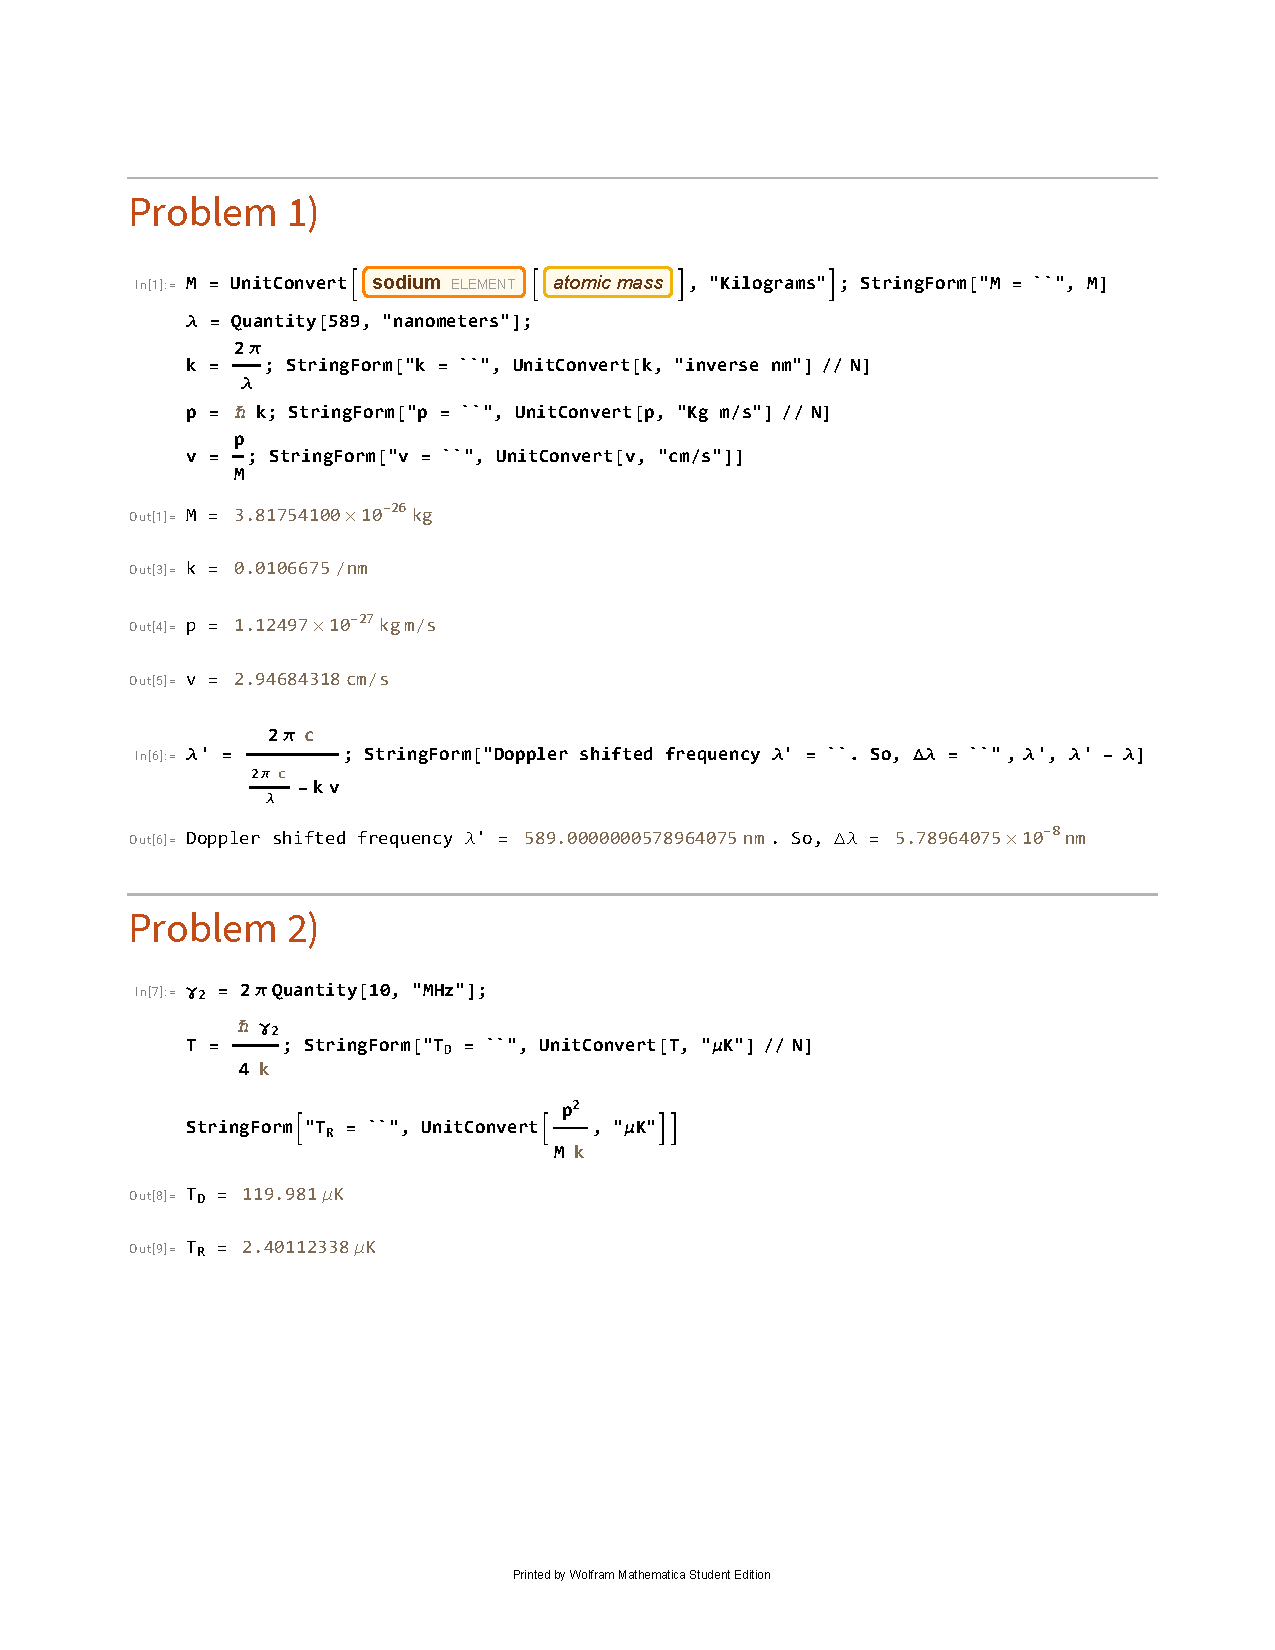
\includepdf[pages=-]{calcs/hw_9.pdf}
\end{document}